%%%%%%%%%%%%%%%%%%%%%%%%%%%%%%%%%%%%%%%%%%%%%%%%%%%%%%%%%%%%%%%%%%%%%%%%%%%%%%%%%%
\begin{frame}[fragile]\frametitle{}
\begin{center}
{\Large Introduction}
\end{center}
\end{frame}

%%%%%%%%%%%%%%%%%%%%%%%%%%%%%%%%%%%%%%%%%%%%%%%%%%%%%%%%%%%%%%%%%%%%%%%%%%%%%%%%%%
\begin{frame}[fragile]\frametitle{Future AI?}
  \begin{itemize}
    \item What are future AI applications like?
	\begin{itemize}
		\item Generative: Generate content like text \& image
		\item Agentic: Execute complex tasks on behalf of human
	 \end{itemize}
	\item How do we empower every developer to build them?: 
	\begin{itemize}
		\item Co-Pilots
		\item Autonomous
	 \end{itemize}	
  \end{itemize}
\end{frame}

%%%%%%%%%%%%%%%%%%%%%%%%%%%%%%%%%%%%%%%%%%%%%%%%%%%%%%%%%%%%%%%%%%%%%%%%%%%%%%%%%%
\begin{frame}[fragile]\frametitle{Examples of Agentic AI}
  \begin{itemize}
  \item Agents mean ACTION
  \item Agentic AI means ACTION using AI, meaning LLM
  \item Examples:
  \begin{itemize}
    \item Personal assistants
    \item Autonomous robots
    \item Gaming agents
    \item Science agents
    \item Web agents
    \item Software agents
  \end{itemize}
    \end{itemize}

\end{frame}


%%%%%%%%%%%%%%%%%%%%%%%%%%%%%%%%%%%%%%%%%%%%%%%%%%%%%%%%%%%%%%%%%%%%%%%%%%%%%%%%%%
\begin{frame}[fragile]\frametitle{Autonomous AI Agents}
  \begin{itemize}
    \item Collaborative approach yields astonishing enhancements in performance and capabilities. Contrasted with using a single AI, such as ChatGPT, in isolation.
    \item Ability to assume distinct roles within a team. Like professionals in various fields.
    \item Each agent contributes specialized expertise to the conversation.
  \end{itemize}
\end{frame}

%%%%%%%%%%%%%%%%%%%%%%%%%%%%%%%%%%%%%%%%%%%%%%%%%%%%%%%%%%%%%%%%%%%%%%%%%%%%%%%%%%
\begin{frame}[fragile]\frametitle{The Blueprint}
  \begin{itemize}
    \item Planning: Reflects on past experiences, offers self-critiques, and breaks down tasks into manageable steps using sub-goal decomposition.
    \item Memory: Utilizes sensory, short-term, and long-term memory for real-time data processing, task-specific information, and retaining knowledge/experiences.
    \item Tools: Equipped with a virtual toolbox, accessing calendars, calculators, search engines, and other resources for versatile problem-solving.
  \end{itemize}
\end{frame}

%%%%%%%%%%%%%%%%%%%%%%%%%%%%%%%%%%%%%%%%%%%%%%%%%%%%%%%%%%%%%%%%%%%%%%%%%%%%%%%%%%
\begin{frame}[fragile]\frametitle{Flow: The Symphony}
  \begin{itemize}
    \item Task Decomposition % : Breaks down tasks into smaller, more manageable components for enhanced efficiency and accuracy.
    \item Model (LLM) Selection % : Chooses the most suitable Large Language Model (LLM) for the task to align actions with desired outcomes.
    \item Task Execution leveraging planning, memory, and tools.
    \item Response Generation % : Generates contextually relevant and accurate responses, be it drafting a report, answering questions, or making decisions.
  \end{itemize}
\end{frame}

%%%%%%%%%%%%%%%%%%%%%%%%%%%%%%%%%%%%%%%%%%%%%%%%%%%%%%%%%%%%%%%%%%%%%%%%%%%%%%%%%%
\begin{frame}[fragile]\frametitle{Agentic Frameworks' Needs}

  \begin{itemize}
  \item Intuitive unified agentic abstraction
  \item Flexible multi-agent orchestration
  \item Effective implementation of agentic design patterns
  \item Support diverse application needs
    \item  Handle more complex tasks / Improve response quality
	\item Easy to understand, maintain, extend Modular composition, Natural human participation, Fast \& creative experimentation
	  \item Agentic Abstraction: Unify models, tools, human for compound AI systems

  \end{itemize}
\end{frame}

%%%%%%%%%%%%%%%%%%%%%%%%%%%%%%%%%%%%%%%%%%%%%%%%%%%%%%%%%%%%%%%%%%%%%%%%%%%%%%%%%%
\begin{frame}[fragile]\frametitle{Multi-Agent Orchestration}


\begin{columns}
    \begin{column}[T]{0.6\linewidth}

		  \begin{itemize}
		  \item Static/dynamic
		  \item Context sharing/isolation
		  \item Cooperation/competition
		  \item Centralized/decentralized
		  \item Intervention/automation
		  \end{itemize}

    \end{column}
    \begin{column}[T]{0.4\linewidth}

		\begin{center}
		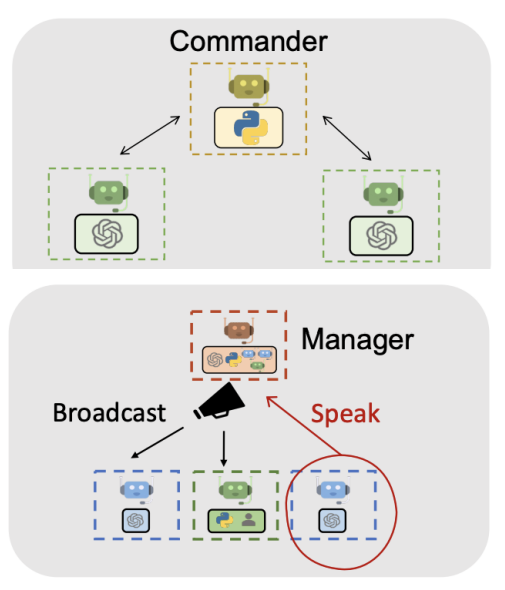
\includegraphics[width=\linewidth,keepaspectratio]{autoagent4}
		\end{center}
	
    \end{column}
  \end{columns}
  
  

\end{frame}

%%%%%%%%%%%%%%%%%%%%%%%%%%%%%%%%%%%%%%%%%%%%%%%%%%%%%%%%%%%%%%%%%%%%%%%%%%%%%%%%%%
\begin{frame}[fragile]\frametitle{Popular Agentic Frameworks}

  \begin{itemize}
    \item BabyAGI: Pioneering AI learning system.
    \item AutoGPT: Automates content generation.
    \item GPT Engineer: Assists in coding and software development.
	\item Langraph: Graph-based control flow
	\item CrewAI: High-level static agent-task workflow
    \item AutoGen: Dialog based planning and execution
  \end{itemize}
\end{frame}

